% !TeX root = ../main.tex

\begin{frame}
  \frametitle{The Idea of Homology}

  \begin{textblock*}{11cm}(1cm,2cm)
    \only<1>{{\small
      \begin{itemize}
        \item $\hom_0$: connected components,
        \item $\hom_1$: loops,
        \item $\hom_2$: voids.
      \end{itemize}}}
    \only<2>{Betti numbers $\beta_k := \mathbf{dim}~\hom_k$}
    \only<3,4>{{\small Elements are equivalence classes of \emph{homologous} cycles.}}
  \end{textblock*}

  \begin{textblock*}{3cm}(1cm,3cm)
    \only<2>{{\small \[\beta_0 = 1\]}}
  \end{textblock*}
  \begin{textblock*}{3cm}(5.75cm,3cm)
    \only<2>{{\small $\beta_0 = 1$\\$\beta_1 = 1$}}
  \end{textblock*}
  \begin{textblock*}{3cm}(9.5cm,3cm)
    \only<2>{{\small $\beta_0 = 1$\\$\beta_1 = 0$\\$\beta_2 = 1$}}
  \end{textblock*}

  \begin{textblock*}{12cm}(1cm,4.5cm)
    \includegraphics<1,2>[trim=100 100 100 100, clip, width=0.3\textwidth]{figures/component}
    \includegraphics<1,2>[trim=100 100 100 100, clip, width=0.3\textwidth]{figures/loop}
    \includegraphics<1,2>[trim=100 100 100 100, clip, width=0.3\textwidth]{figures/void}
  \end{textblock*}
  \begin{textblock*}{8cm}(1.5cm,4.25cm)
    \includegraphics<3>[trim=200 400 200 400, clip, width=0.7\textwidth]{figures/torus1}
    \includegraphics<4>[trim=200 400 200 400, clip, width=0.7\textwidth]{figures/torus2}
  \end{textblock*}
  \begin{textblock*}{4cm}(8.5cm,6cm)
    \only<3,4>{{\small $\beta_0 = 1$\\$\beta_1 = 2$\\$\beta_2 = 1$}}
  \end{textblock*}
\end{frame}


\begin{frame}
  \frametitle{Homology of Simplicial Complexes}

  \begin{textblock*}{11cm}(1cm,2cm)
    \begin{small}
      The \emph{boundary} of a $k$-simplex is a $(k-1)$ cycle.\vspace{1ex}

      \only<2>{A $k$-cycle in has non-trivial homology if it is not the boundary of a $(k+1)$-\emph{chain}.}
    \end{small}
  \end{textblock*}

  \begin{textblock*}{11cm}(1cm,4.5cm)
    
\includegraphics[trim=0 0 -400 0, clip, width=0.3\textwidth]{figures/edge_bdy}
    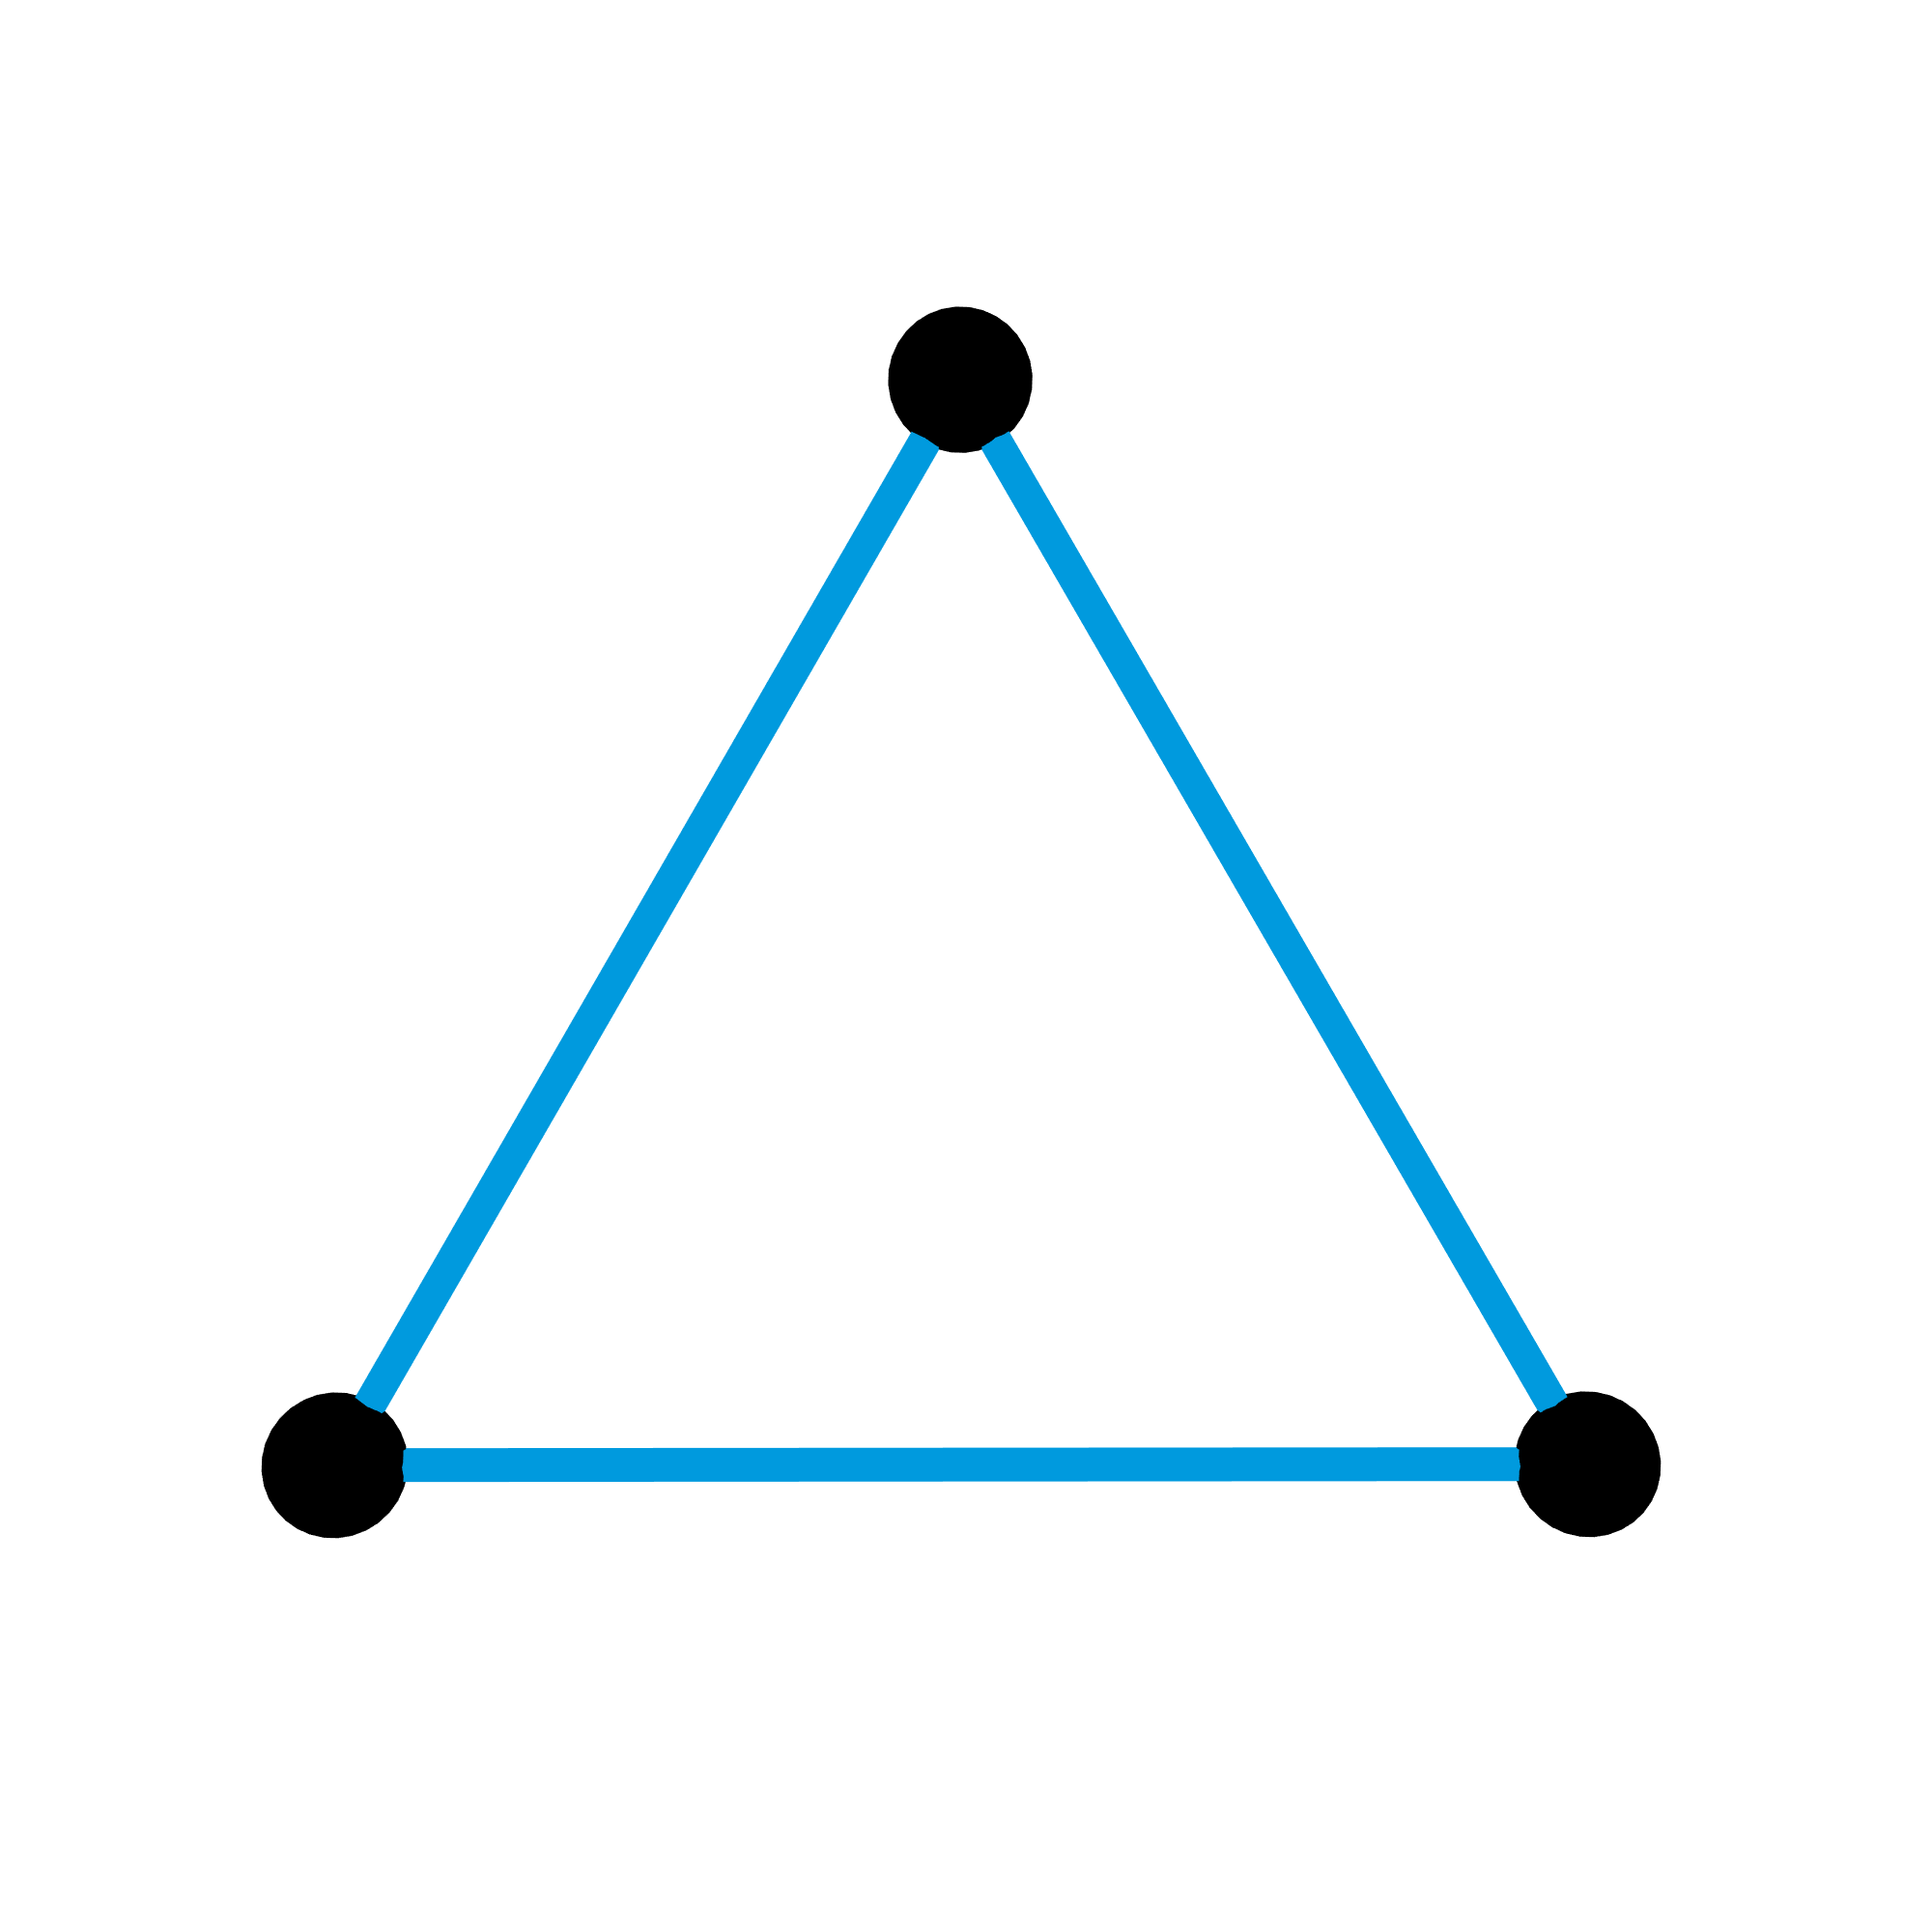
\includegraphics[trim=0 0 -200 0, clip, width=0.3\textwidth]{figures/tri_loop}
    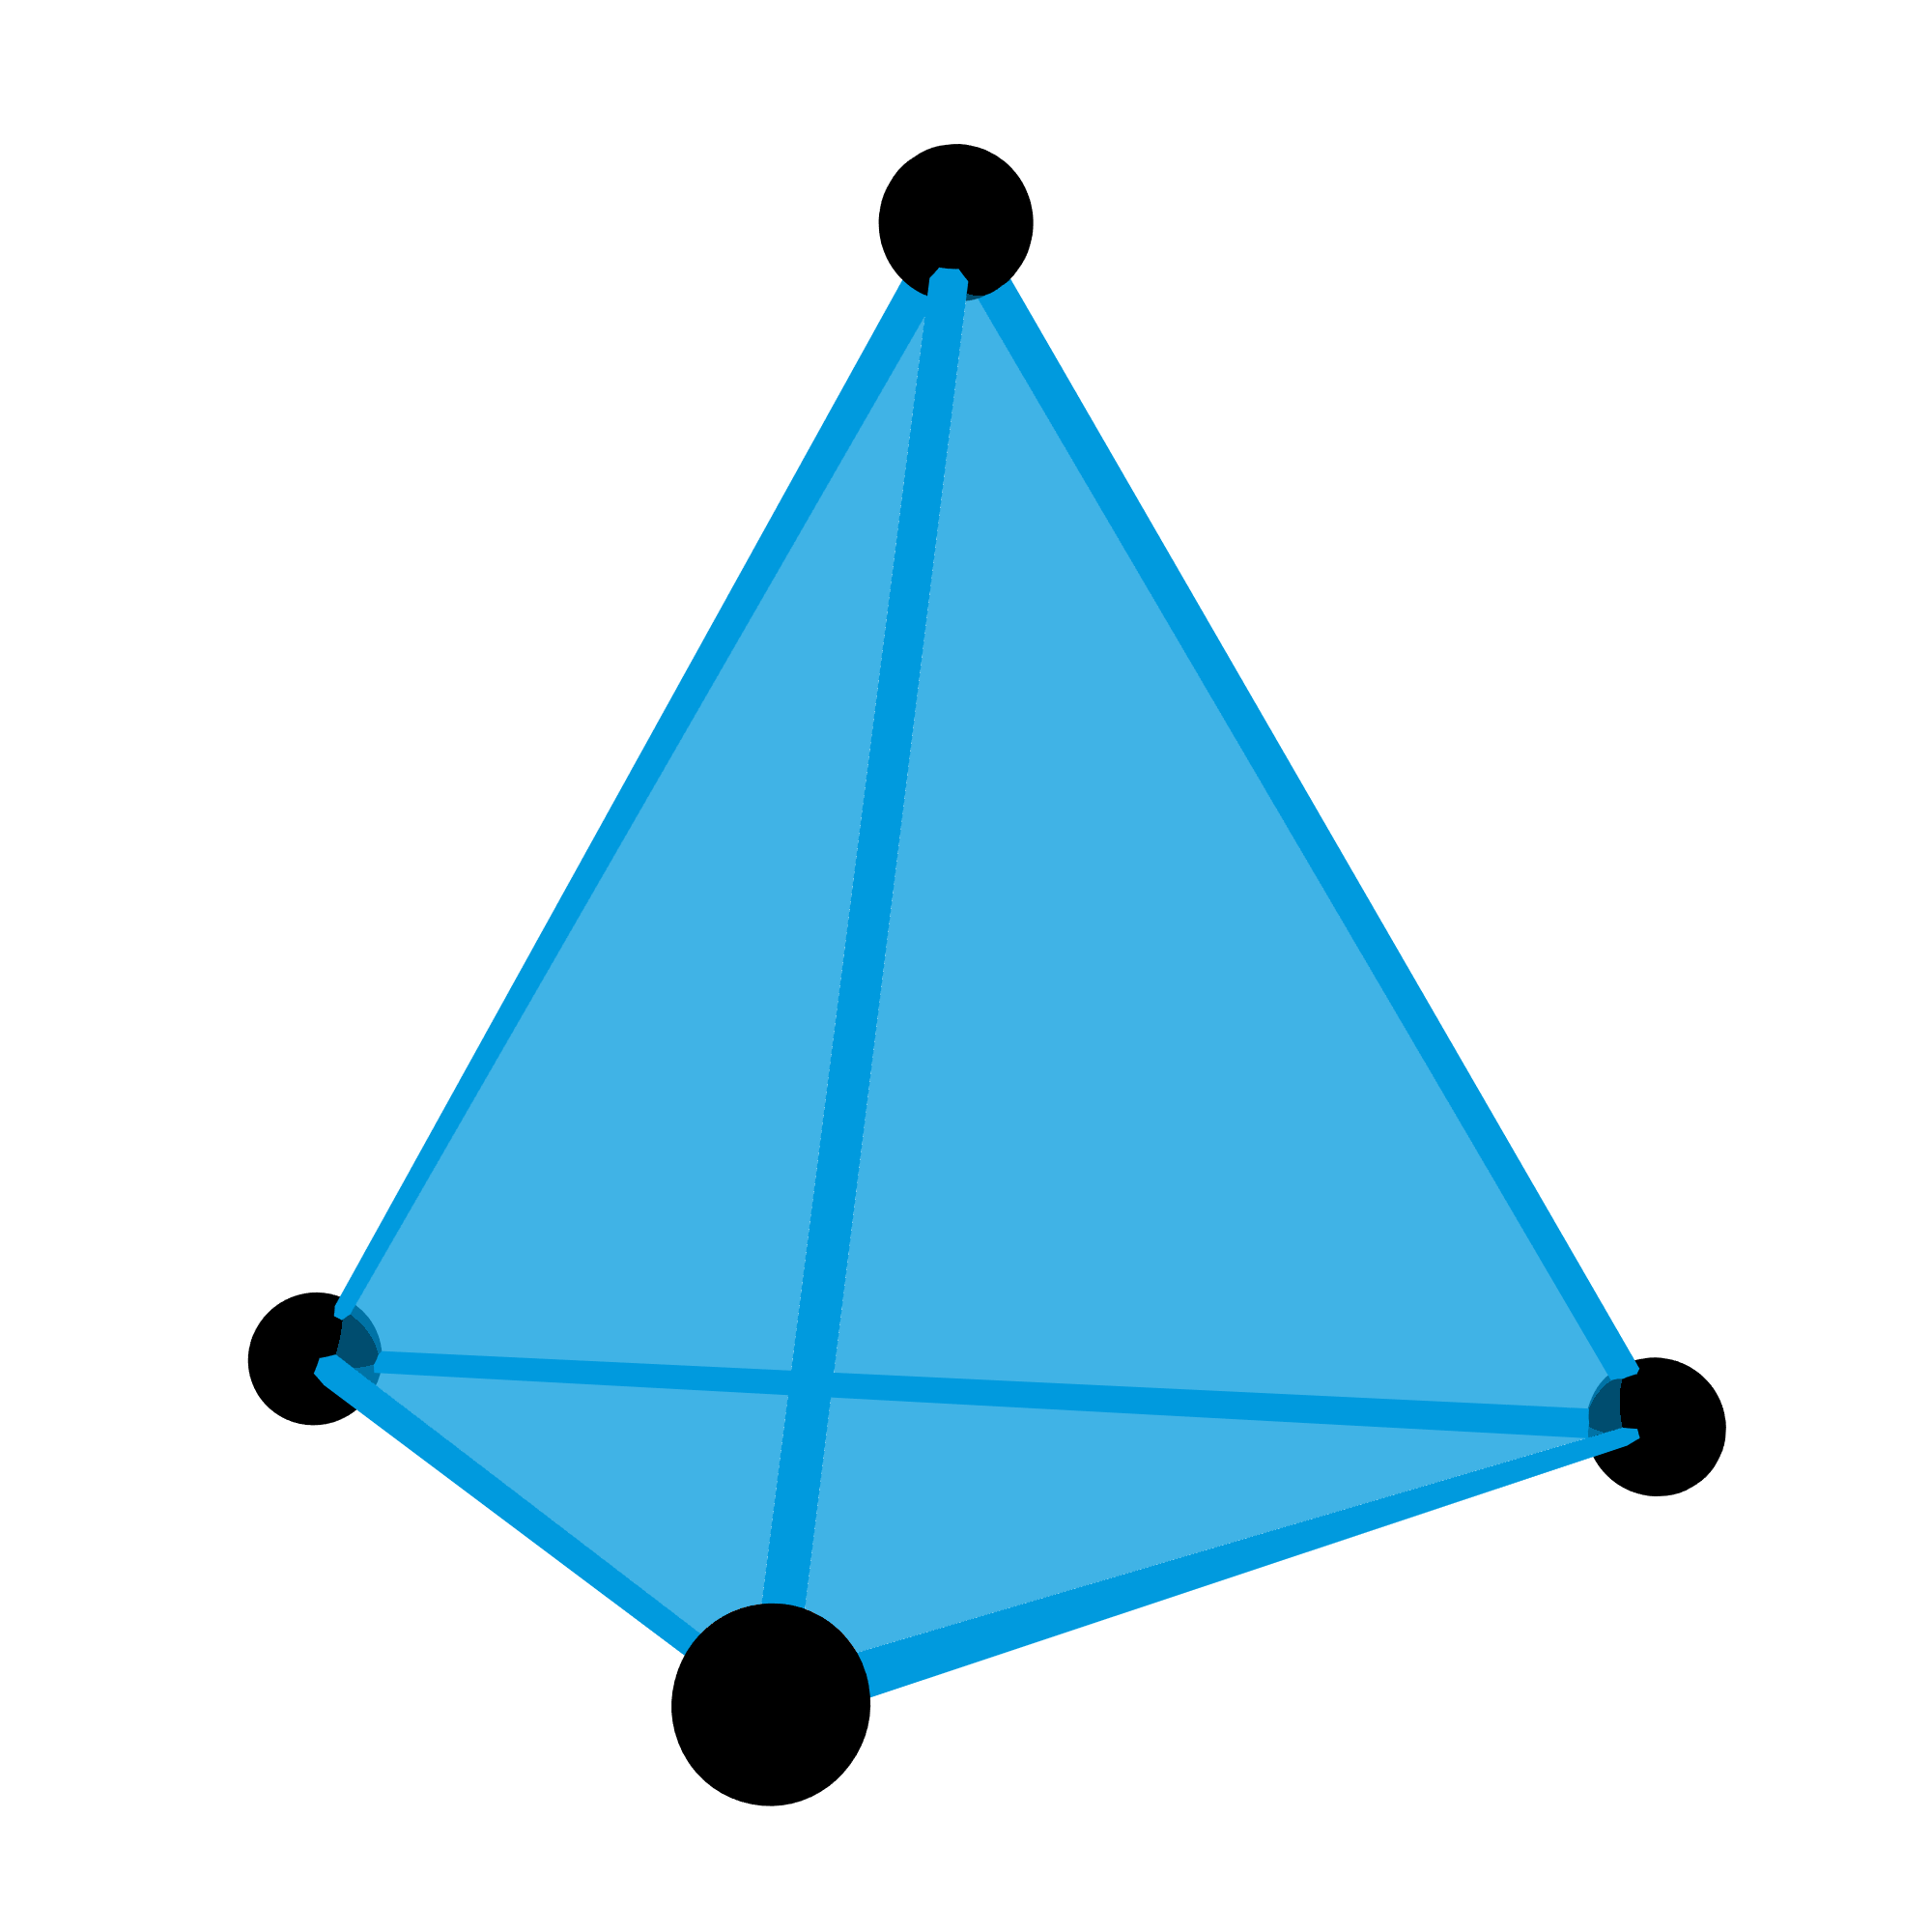
\includegraphics[trim=-200 0 0 0, clip, width=0.3\textwidth]{figures/tet_void}
  \end{textblock*}
\end{frame}
